%!TEX root=main.tex
\chapter{Background} \label{cap:conceitos}

This chapter provides an overview on fully homomorphic encryption, on CKKS, with a particular focus on its client-side operations and a brief discussion of the server-side operations. It also introduces the more relevant architectural features of the ARMv8 platform and the OpenMP programming model used throughout this work.

\section{Fully Homomorphic Encryption}

Homomorphic Encryption (HE) is a cryptographic scheme that enables computations to be performed directly on encrypted data while preserving the equivalence between the results of these computations and those obtained by applying the same operations to the corresponding plaintext data. This property allows an untrusted third party to process sensitive information without gaining access to its underlying content. The typical workflow involves encrypting sensitive data on the client side, transmitting the resulting ciphertext to a server, performing the required homomorphic operations on the encrypted data, and returning the resulting ciphertext to the client for decryption, as illustrated in Figure~\ref{fig:fhe_overview}.

\begin{figure}
    \centering
    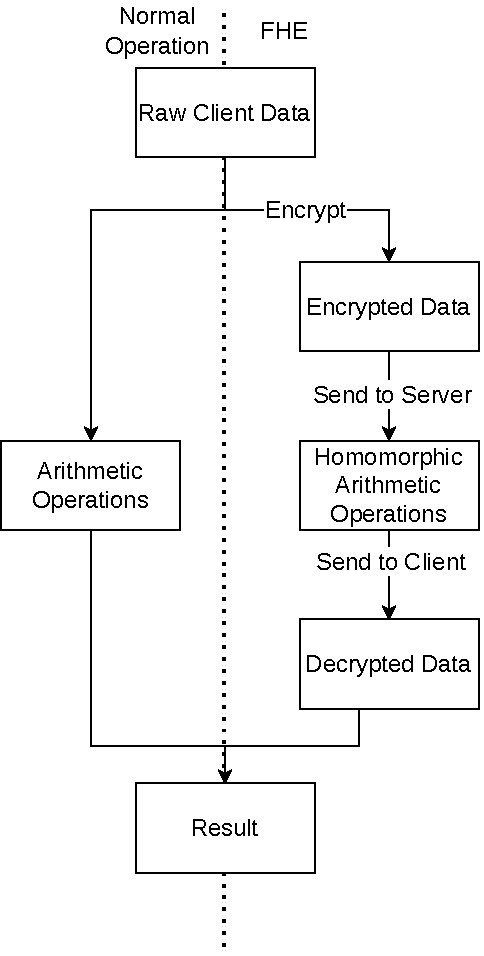
\includegraphics[width=0.4\linewidth]{Images/FHE.pdf}
    \caption{HE Overview}
    \label{fig:fhe_overview}
\end{figure}

HE schemes typically support two fundamental arithmetic operations: addition and multiplication. These operations serve as building blocks for more complex computations, including division, logical operations (e.g., AND and XOR), and the evaluation of non-linear functions, such as trigonometric and exponential functions. However, several  schemes introduce noise into ciphertexts as part of their underlying construction. Although this noise does not affect the correctness of decryption as long as it remains within certain bounds, successive homomorphic operations can increase its magnitude and eventually compromise the correctness of the decrypted result. Another major limitation of  is its computational overhead, as homomorphic operations can be significantly more expensive than their counterparts on plaintext data. In particular,  operations have been reported to be approximately $100\times$ to $1000\times$ slower than equivalent operations performed on unencrypted data~\cite{martins2017survey}.

Furthermore, HE schemes can be classified into three subcategories: Partially Homomorphic Encryption (PHE), Leveled Fully Homomorphic Encryption (Leveled FHE), and Fully Homomorphic Encryption (FHE). PHE schemes support a single type of operation, either addition or multiplication, which can be performed an unlimited number of times without compromising the integrity of the encrypted data. Leveled FHE schemes support both addition and multiplication but impose a limit on the computational depth of the operations that can be performed. Finally, FHE schemes support both operations an unlimited number of times, without compromising the integrity of the encrypted data.

\section{CKKS}

CKKS~\cite{cheon2017homomorphic} is an approximate  fully homomorphic encryption scheme designed to support arithmetic operations on vectors of complex numbers. Due to its approximate nature, the decrypted result may differ from the exact value, with the approximation error depending on the operations performed on the ciphertexts. This error can be bounded and controlled to ensure that the decrypted result remains within an acceptable range of the expected value. When properly managed, such approximation errors are generally acceptable in many applications involving real or complex numbers, as these applications often tolerate small numerical deviations. Furthermore, these deviations are consistent with the numerical imprecision inherent in the finite-precision representation of real numbers in computers.

Given a vector of complex numbers, referred to as a \emph{slot vector}, CKKS encodes them into a vector of integer values and encrypts this second vector into a ciphertext. Homomorphic operations can then be performed directly on the ciphertext of integer numbers, without decrypting it. After decryption and decoding, the resulting slot vector approximately corresponds to the result that would have been obtained by performing the same operations directly on the original complex-valued vectors.

The operations involved in CKKS can be broadly divided into client-side and server-side operations. The client-side operations include parameter generation, key generation, encode, encryption, decode, and decryption. The server-side operations include ciphertext-ciphertext arithmetic (addition and multiplication), ciphertext-plaintext arithmetic (addition and multiplication), ciphertext rotation, and bootstrapping. While this work primarily focuses on the implementation and optimization of the client-side operations, the main server-side operations - less bootstraping - are also implemented to enable complete end-to-end execution between the client and server.

\subsection{Overview}

The homomorphic operations in CKKS are performed over the polynomial ring $\mathbb{Z}_Q[X]/(X^n+1)$, where each polynomial has degree less than $n$ and integer coefficients represented by elements of $\mathbb{Z}_Q$. These coefficients are typically represented by integers in the centered interval $\left\{-\frac{Q-1}{2}, \ldots, -1, 0, 1, \ldots, \frac{Q-1}{2}\right\}$, assuming that $Q$ is odd. To ensure that the coefficients remain within this range, arithmetic operations are followed by modular reduction. Specifically, coefficient-wise addition and multiplication are performed modulo $Q$, while polynomial multiplication is carried out modulo $X^n+1$ to reduce the resulting polynomial to degree less than $n$. In the original CKKS construction, the ciphertext modulus is defined as $Q = q_0 \Delta^L$, where $q_0$ is the initial modulus, $\Delta$ is the scaling factor, and $L$ denotes the maximum multiplicative depth supported by the modulus chain.

As illustrated in Figure~\ref{fig:ckks_overview}, given an input slot vector $v \in \mathbb{C}^{\frac{n'}{2}}$, the client first encodes $v$ into a plaintext polynomial $m \in \mathbb{Z}_Q[X]/(X^n+1)$. The plaintext is then encrypted using the secret key $s$ into a ciphertext $c$. The resulting ciphertext is transmitted to the server, which can perform homomorphic operations on it without access to the underlying plaintext. After the computation is completed, the server returns the resulting ciphertext to the client. The client decrypts and decodes this ciphertext to obtain an output slot vector $v'$, which approximately corresponds to the result that would have been obtained by performing the same computation directly on the original input vector.

\begin{figure}
    \centering
    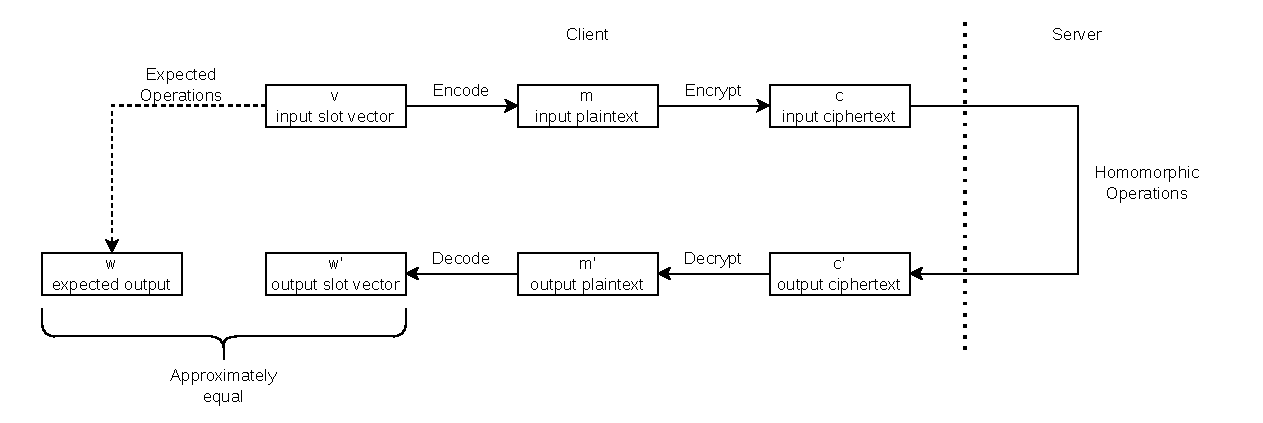
\includegraphics[width=1\linewidth]{Images/CKKS_Overview.pdf}
    \caption{CKKS Client-Side Overview}
    \label{fig:ckks_overview}
\end{figure}

CKKS is an approximate homomorphic encryption scheme because its encoding and encryption procedures introduce noise and approximation errors into the represented data. During encoding, the input complex values are scaled and mapped to a finite-precision representation, introducing a quantization error. Encryption additionally introduces noise as part of the underlying lattice-based encryption construction. These errors propagate through homomorphic computations and generally increase as additional operations are performed.

In particular, ciphertext multiplication significatly increases the noise. To control this growth, CKKS employs a rescaling step after a ciphertext multiplication. Rescaling reduces the ciphertext modulus by removing one multiplicative level.

Once the available levels have been exhausted, further multiplications cannot be performed while maintaining the required precision and security properties. To support computations with a greater multiplicative depth, CKKS provides a bootstrapping procedure that refreshes the ciphertext by homomorphically reducing its accumulated noise and restoring its available computation levels~\cite{cheon2018bootstrapping}.

Therefore, the responsibilities of the client application include configuring the CKKS parameters, generating the required keys, encoding and encrypting the user's input slot vectors, and decrypting and decoding the results returned by the server. The server, in turn, performs the desired computations in the homommorphic domain.

\subsubsection{RNS Construction}

The original formulation of CKKS presents a significant performance challenge when supporting computations with a large multiplicative depth. Since bootstrapping is computationally expensive, it is desirable to choose a sufficiently large modulus to allow multiple homomorphic multiplications to be performed before bootstrapping is required. However, directly representing such a large modulus using conventional integer arithmetic introduces substantial computational overhead. In particular, for practical parameter sets, the ciphertext modulus can be significantly larger than the native word size of processors (typically 32 or 64 bits), requiring multi-precision or long-word arithmetic. Such operations are considerably more expensive than arithmetic over native machine words.

Therefore, to solve this problem another construction for the moduli $Q$ is proposed, instead of $Q=q_0\Delta^L$, we use $Q=q_0q_1\ldots q_L$ such that $q_i$ is a prime and $q_i\approx\Delta$, for $1\leq i\leq L$ and $q_i \not\equiv q_j$, for $1\leq i, j \leq L$ and $i \not\equiv j$ . Then, we can use the Chinese Remainder Theorem (CRT) which proofs that for any number $b\in\mathbb{Z}_Q$ can be unique represented by the $L+1$ sequence $b_0, b_1, \ldots, b_L$, such that $b \equiv b_i \bmod q_i$ and $-\frac{q_i}{2} < b_i < \frac{q_i}{2}$. Using this representation all addition and multiplication operations moduli $Q$ can instead be performed individually into each $L+1$ elements. Since each $q_i$ can be selected to fit within the native word size of the target processor, the expensive multi-precision operations can be replaced by several smaller integer operations~\cite{cheon2018faster}.

One major drawback of this technique is that division is more complicated than element-wise addition and multiplication. The general approach is to reconstruct the integer represented by the residues modulo \(Q\) and then perform the division using arbitrary-precision arithmetic, which is computationally expensive. Fortunately, in our setting, we are interested in only two special cases in which division can be implemented much more efficiently.

First, when the divisor \(Y\) is coprime to \(Q\), i.e., \(\gcd(Y,Q)=1\), division can be implemented as element-wise multiplication by the modular inverse of \(Y\) modulo each residue modulus \(q_i\), namely \(Y_i^{-1} \bmod q_i\). Second, when \(Y=q_t\) for some \(t\), where \(q_t\) is one of the moduli dividing \(Q\), each residue can be computed by subtracting the corresponding residue from the modulus \(q_t\) and then multiplying by \(Y_i^{-1} \bmod q_i\).

\subsubsection{Polynomial Operations}
\label{ckks:ops}

The schoolbook methods for $n$-degree polynomial addition and multiplication require $\mathcal{O}(n)$ and $\mathcal{O}(n^2)$ operations, respectively, however since $n$ is very large for usual CKKS parameters ($2^{13} \leq n \leq 2^{20}$) a $O(n^2)$ algorithm is very expensive. Fortunately, for polynomial multiplications in $\mathbb{Z}_{q_i}[X]/(X^n+1)$ we can reduce its computational cost to $\mathcal{O}(n \log n)$ by applying the Number Theoretical Transform (NTT).

First, we convert a polynomial to the NTT domain, in which the schoolbook polynomial multiplication becomes a point-wise multiplication in $\mathcal{O}(n)$ operations, and then we convert the polynomial back to the original domain by employing the Inverse NTT (INTT). %By using the } transformations we can perform the NTT and INTT in $O(n \log n)$ time, respectively and the point-wise multiplication in $O(n)$ operations.

More formally, the NTT in $X^n+1$ maps the input vector $v = (v_0, v_1, \ldots, v_{n-1})$ to the output vector $w = (w_0, w_1, \ldots, w_{n-1})$ according to  $w_k = \sum^{n-1}_{j=0}v_j\alpha_i^{(2j+1)k} \bmod q_i, 0 \leq k < n$, where $\alpha_i$ is an $2n$-th primitive root of $q_i$, such that $\alpha_i^{2n} \equiv 1 \mod q_i$ and $\alpha^j_i \not\equiv 1 \mod q_i$, $1 \leq j < 2n$. Similarly, the INTT maps $w$ into $v$ as $v_k = \frac{1}{n} \sum^{n-1}_{j=0}w_j\alpha_i^{-(2j+1)k} \bmod q_i, 0 \leq k < n$.

A naive implementation of this construction requires $\mathcal{O}(n^2)$ operations, yielding the same asymptotic complexity as the schoolbook method and thus offering no computational advantage. However, more efficient algorithms, such as Cooley--Tukey (CT)~\cite{cooley1965algorithm} and Gentleman--Sande (GS)~\cite{gentleman1966fast}, reduce the complexity to $\mathcal{O}(n\log n)$. These algorithms produce output arrays whose elements are arranged in bit-reversed order, as illustrated in Figure~\ref{fig::ntt}. CT-NTT transforms the input polynomial in normal order into the output polynomial in the bit-reverse order, while the GT-INTT receives this bit-reversed output and transforms back to the normal order, so the bit-reversing operations are automatically canceled and no extra computation is required.

\begin{figure}
    \centering
    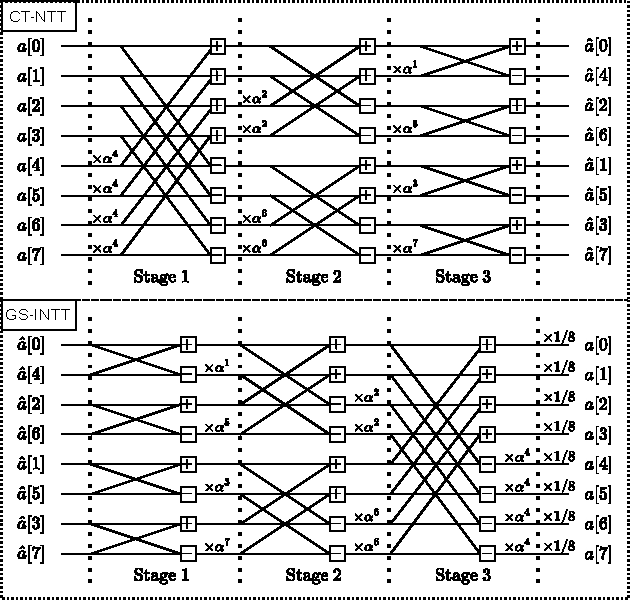
\includegraphics[width=1\linewidth]{Images/NTT-CT-GS.pdf}
    \caption{CT-NTT and GS-INTT for the vector $a$ with 8 elements.}
    \label{fig::ntt}
\end{figure}

Moreover, CKKS supports left rotations of the input slot vector by $h$ positions, which are equivalent to mapping the coefficient of $X^i$ to the coefficient of $X^{5^h i} \bmod X^n + 1$. %The operation is described in more details in~\ref{ckks:client}.

\paragraph{doubleCRT}

Furthermore, \cite{cheon2018full} defines the \textbf{doubleCRT} representation, in which each ciphertext is stored as $L+1$ residues in the NTT domain. Consequently, sequences of ciphertext additions and multiplications can be performed directly in the NTT domain without requiring additional NTT transformations, allowing each operation to be performed in $\mathcal{O}(n)$ complexity time. However, ciphertext rotations and divisions by one of the moduli $q_i$ require the ciphertext to be transformed back to the original domain, where the corresponding operation can be applied, followed by a transformation back to the NTT domain. These NTT and inverse NTT transformations increase the complexity of a rotation and a division to $\mathcal{O}(n\log n)$. 

Therefore, the \textbf{doubleCRT} representation is particularly well suited to workloads dominated by ciphertext additions and multiplications, as these operations can be performed directly in the NTT domain. In contrast, workloads involving frequent rotations and divisions by one of the moduli $q_i$ incur a significant additional computational cost due to the required domain transformations.

\subsubsection{Constant-Time Reductions}
\label{ckks:cte_red}

Our coefficient-level operations require modular reduction after both addition and multiplication. A straightforward approach would be to use the hardware integer division or remainder instructions to perform these reductions. However, the execution time of such instructions can depend on the input operands on some processor architectures, including in the ARMv8 processors such as the Arm Cortex-A55~\cite{arm2023cortexa55}.

As discussed in Section~\ref{cap:especificacao}, one of the requirements of this project is to ensure constant-time execution for operations involving secret data. Therefore, hardware instructions with potentially input-dependent execution times cannot be relied upon for modular reduction. Instead, we employ constant-time modular arithmetic techniques, namely Montgomery multiplication~\ref{background::math::montgomery} and Barrett reduction~\cite{barrett1986implementing}.

\paragraph{Montgomery Multiplication}

Algorithm~\ref{background::math::montgomery} describes the Montgomery modular multiplication algorithm. Let $R = 2^\ell$, where $\ell$ is a positive integer, and let $q$ be a positive integer such that $\gcd(R,q)=1$. Furthermore, let $\bmod^{\pm}$ denote the modular reduction operation over the symmetric interval $\left[\frac{-(q-1)}{2}, \frac{(q-1)}{2}\right]$.

Given integers $a$ and $b$, Montgomery multiplication computes $c = abR^{-1} \bmod q$ with $c \in (-q, q)$. To obtain the conventional product $ab \bmod q$, one can perform a subsequent Montgomery multiplication by $R^2$, yielding $abR^2R^{-2} \equiv ab \bmod q$. When multiple arithmetic multiplications are performed successively, it is more efficient to keep the operands and intermediate results in the Montgomery domain. This is typically achieved by converting the operands into this domain using Montgomery multiplication by $R^2$, so that each operand is represented as $aR \bmod q$. Subsequent Montgomery multiplications preserve this representation, maintaining the factor $R$ in the intermediate results. Only after the final multiplication is a Montgomery multiplication by $1$ required to recover the conventional representation, effectively removing the factor $R$.

Furthermore, when one operand $b$ is a constant, its Montgomery representation, $bR \bmod q$, can be precomputed and stored. Multiplying $a$ by this precomputed value using Montgomery multiplication directly yields $ab \bmod q$, without requiring additional conversion operations.

\begin{algorithm}[!ht]
\caption{Montgomery Modular Multiplication}
\label{background::math::montgomery}
\footnotesize
\begin{algorithmic}[1]
\Procedure{\texttt{montgomery\_multiplication}}{Integers a, b; $\frac{-Rq}{2} \leq a, b < \frac{Rq}{2}$, $R=2^\ell$}
\State $m = ab q^{-1} \mod^{\pm} R$\;
\State $t = m q \gg \ell $\;
\State $r = (ab \gg \ell) - t$\;
\State \Return $r$, where $r = abR^{-1} \mod^{\pm} q, r \in (-q, q)$ \;
\EndProcedure
\end{algorithmic}
\end{algorithm}

\paragraph{Barrett Reduction}

The Barrett reduction algorithm for $R = 2^\ell$ and an odd modulus $q$ is presented in Algorithm~\ref{background::math::barret}, where $\lfloor \cdot \rfloor$ denotes the floor operation. Unlike Montgomery multiplication, which computes the product of two operands while incorporating a factor of $R^{-1}$, Barrett reduction directly reduces a single value modulo $q$ without introducing additional terms into the result. However, whereas Montgomery arithmetic can be implemented entirely using single-width arithmetic, Barrett reduction may require double-width arithmetic for certain intermediate values.

\begin{algorithm}[!ht]
\caption{Barrett Reduction}
\label{background::math::barret}
\footnotesize
\begin{algorithmic}[1]
\Procedure{\texttt{barrett\_reduction}}{Integer a; $\frac{-R}{2}  \leq a < \frac{R}{2}, R  = 2^\ell, \text{ odd } q < R$ and $v = \left\lfloor \frac{R}{q} \right\rceil$}
\State $m = \lfloor a v/ 2^\ell \rceil $\;
\State $r = a - m q$\;
\State \Return $r$, where $r = a \mod^\pm q, r \in (-q, q)$\;
\EndProcedure
\end{algorithmic}
\end{algorithm}

\subsubsection{Ring Learning With Errors}

The security of CKKS relies on the hardness of the Ring Learning with Errors (RLWE) problem. In the CKKS setting, let $A$ be a polynomial whose coefficients are sampled uniformly from $\mathbb{Z}_Q$, let $S$ be a secret polynomial with coefficients sampled uniformly from the ternary set $\{-1,0,1\}$, let $E$ be a small error polynomial whose coefficients are sampled from a discrete Gaussian distribution and $\Delta M$ the plaintext polynomial. Given these polynomials, an RLWE sample can be expressed as $\text{RLWE}_S(\Delta M + E) = (A,B) = \left(A,-AS + \Delta M + E\right) \pmod Q$. The hardness of the RLWE problem relies on the difficulty of recovering $\Delta M + E$ and $S$ from ($A$, $B$).

Similarly to the RLWE problem, the Learning With Errors (LWE) and Module Learning With Errors (MLWE) problems provide alternative mathematical foundations for constructing lattice-based cryptographic schemes. In the LWE variant, given a uniformly sampled vector \(a \in \mathbb{Z}_q^n\), where \(n\) is a positive integer and \(q\) is a prime modulus, a secret key \(s \in \mathbb{Z}_q^n\), and a small error term \(e\), the encryption of a message \(m\) can be expressed using a scaling factor \(\Delta\), such that \(\Delta m + e < q\). The resulting ciphertext is defined as $\text{LWE}_s(\Delta m + e) = (a,b) = \left(a,-a^Ts + \Delta m + e\right) \pmod q$ where the error term satisfies \(|e| < \Delta\). As in RLWE, the security of LWE relies on the computational difficulty of recovering the secret key \(s\) or the original message from $(a, b)$.

The Module Learning With Errors (MLWE) problem extends the LWE framework by introducing a module structure over a polynomial ring, combining features of LWE and Ring Learning With Errors (RLWE). Let \(R_q = \mathbb{Z}_q[x]/X^n+1)\), where $n$ is a positive integer and $q$ a prime, and let \(k\) be a positive integer representing the module rank. Given a uniformly sampled vector \(a \in R_q^k\), a secret key \(s \in R_q^k\), and a small error polynomial \(e \in R_q\), an MLWE ciphertext component can be expressed as $b = -\langle a,s\rangle + \Delta m + e \pmod q$, where \(\langle a,s\rangle = \sum_{i=1}^{k} a_i s_i\) denotes the inner product over \(R_q\), and \(m\) is the encoded message. The corresponding ciphertext is therefore $\text{MLWE}_s(\Delta m + e) = (a,b)$. The security of MLWE relies on the difficulty of recovering the secret vector \(s\) or the original message from $(a, b)$. %By adjusting the module rank \(k\), MLWE provides a flexible balance between the algebraic efficiency of RLWE-based constructions and the security properties associated with LWE, making it a useful foundation for modern lattice-based cryptographic schemes.

\subsubsection{Converting slot vectors into polynomials}
\label{ckks::convert}

The input vector slot is defined in $\mathbb{C}^{\frac{n'}{2}}$, while the polynomials are defined in $\mathbb{Z}_Q[X]/(X^n+1)$, with both $n'$ and $n$ being powers of two and $n' \leq n$, so we need a method to convert the slot vectors into the polynomials. In CKKS, we employ the Discrete Fourier Transform (DFT) and its inverse (IDFT) for this operation. The DFT and IDFT are the analogous transforms of the NTT and INTT, respectively, operating over $\mathbb{C}^{\frac{n'}{2}}$ with time complexity $O(n' \log n')$.

Moreover, to support ciphertext rotation operations, the ordering of the powers of $\alpha$ must be rearranged, mapping $\alpha^{2j+1}$ to $\alpha^{5^j}$ when $j < \frac{n'}{2}$ and to $\alpha^{-5^j}$ when $j \geq \frac{n'}{2}$. However, in this construction, the primitive-root access pattern illustrated in Figure~\ref{fig::ntt} changes from blocked to interleaved at a certain stage. Since this structure is typically implemented using three nested loops (stage, permutation block, and vector), this change significantly increases the computational cost. In the blocked pattern, primitive roots can be loaded in the middle loop because they depend only on the permutation block and remain constant across the inner loop iterations. In contrast, the interleaved pattern makes primitive-root selection dependent on the current element, requiring the roots to be loaded in the innermost loop. %This additional memory-access overhead reduces the efficiency of the implementation.

Furthermore, the IDFT operates on the slot vector in natural order, unlike the INTT input shown in Figure~\ref{fig::ntt}, which is in bit-reversed order. Consequently, the permutation patterns must be reversed relative to those illustrated in Figure~\ref{fig::ntt}. As a result, the GS-IDFT and CT-DFT follow the same permutation patterns as the CT-NTT and GS-INTT, respectively.

% TODO: Literature review
\subsection{Client-Side Operations}
\label{ckks:client}

This subsection describes the main client-side operations of CKKS: parameter generation, key generation, encode, decode, encryption, and decryption. Key generation is presented last, as it involves more complex operations than the other procedures.

\subsubsection{Parameter Generation}

The client application should provide an interface for configuring the CKKS parameters according to two scenarios: minimum and complete. In the complete scenario, the user specifies all the parameters: the slot vector size $n'$, the scale factor $\Delta$, the multiplicative depth $L$, the polynomial degree $n$, and the modulus chain $q_0, q_1, \ldots, q_L$. In the minimum scenario, the user specifies only the slot vector size $n'$, the scale factor $\Delta$, the multiplicative depth $L$, and the bit length of the initial modulus, $\lfloor \log_2 q_0 \rfloor$, while the remaining parameters ($n$ and the modulus chain) are computed by the application.

Furthermore, in both scenarios the applicaton is responsible by computing the primitive roots of $\mathbb{C}^{\frac{n'}{2}}$ and $\mathbb{Z}_Q[X]/(X^n+1)$ for the following DFT and NTT operations, respectively.

\subsubsection{Encode}

The encoding procedure transforms the input vector of slots $v$ into the plaintext polynomial $\Delta M$. First, it applies the IDFT to $v$ and maps the real and imaginary components of the output vector to the lower and upper halves of the vector $m' \in \mathbb{R}^{n'}$. Each coefficient $m'_i$ is then multiplied by the scaling factor $\Delta$, and the result is rounded to the nearest integer to obtain the corresponding coefficient of $\Delta M' \in \mathbb{Z_Q}[X]/(X^{n'}+1)$. In particular, $\Delta$ must be chosen such that $-\frac{q_0}{2} < \Delta m'_i < \frac{q_0}{2}$ for all $i$, ensuring that the scaled coefficients remain within the desired range. Finally, $\Delta M$ is obtained as $\Delta M_i = \Delta M'_{in/n'}$, if $(n/n')|i$, otherwise $\Delta M_i = 0$.

\subsubsection{Encryption}
\label{ckks:encrypt}

%Let the Discrete Fourier Transform (DFT) and its inverse (IDFT) be the analogous transforms to the NTT and INTT, respectively, operating over $\mathbb{C}^{\frac{n'}{2}}$ with time complexity $O(n' \log n')$. To support ciphertext rotation operations, the ordering of the powers of $\alpha$ is rearranged, mapping $\alpha^{2j+1}$ to $\alpha^{5^j}$ when $j < \frac{n'}{2}$ and to $\alpha^{-5^j}$ when $j \geq \frac{n'}{2}$.

% TODO: Sparse S
After encoding, the plaintext must be protected with the RLWE construction, which means given a secret key $S$, a uniformly sampled polynomial $A$ and a small error polynomial $E$, the ciphertext $c$ is computed as $c = \text{RLWE}(\Delta M + E)_S = (A, B) =  (A, -AS + \Delta M + E) \bmod Q$.

\paragraph{Polynomial Sampling}

The coefficients of $S$ are uniformly sampled from the ternary distribution $\{-1,0,1\}$, while the coefficients of $E$ are sampled from a centered binomial distribution and the polynomial $A$ is sampled uniformly from $\mathbb{Z}_Q$. In the original mathematical construction of $E$ are sampled from a discrete gaussian sampling. However, discrete Gaussian sampling is well known to be computationally expensive and can introduce quantization issues. A common alternative is therefore to use a centered binomial distribution which can provide the same security properties when its variance is at least as large as that of the corresponding Gaussian distribution. For CKKS, a centered binomial distribution with parameter $k \geq 21$, whose sampling set is $\{-k,\ldots,k\}$, provides sufficient variance. Moreover, $E$ must satisfy the following inequality: $|E|_{\infty}<\frac{\Delta}{2}$, where $|\cdot|_{\infty}$ denotes the infinity norm.

Another implementation challenge is how to perform these samplings efficiently. A common approach is to start from a small true random seed and use an Extendable-Output Function (XOF) to generate a pseudorandom byte stream, which is then processed to obtain samples from the desired distribution. An XOF is a cryptographic primitive that, given a seed, can produce a pseudorandom output of arbitrary length~\cite{stallings2014network}.

\subsubsection{Decryption}
\label{ckks:decrypt}

To decrypt the ciphertext $c=(A,B)$, we define the operation $\text{RLWE}_S^{-1}(c) = \text{RLWE}_S^{-1}((A, B)) = B + AS \equiv \Delta M + E \bmod Q$. Thus, decryption recovers the encoded plaintext polynomial together with the error introduced during encryption. Consequently, the resulting plaintext polynomial is not identical to the original encoded plaintext $\Delta M$.

For the parameter configurations considered in CKKS, the initial modulus $q_0$ and the scale factor $\Delta$ are selected such that a valid ciphertext satisfies $|\Delta M + E|_{\infty} < \frac{q_0}{2}$. Under this condition, the coefficients can be recovered unambiguously from their representation modulo $q_0$. Therefore, when the ciphertext is stored in the \textbf{doubleCRT} representation, the decryption operation only needs to evaluate the corresponding expression for the $q_0$ residue to reconstruct the plaintext polynomial.

\subsubsection{Decode}
\label{ckks:decode}

The decoding procedure divides the resulting polynomial by the scale factor $\Delta$, and applies the DFT to map the polynomial coefficients back to the slot-vector domain. If the accumulated error remains respecting $|E|_{\infty} < \frac{\Delta}{2}$ after the server-side computations, the decoded vector approximately corresponds to the expected result. The magnitude of the approximation error depends on the accumulated noise and on the scale factor used throughout the computation.

\subsubsection{Keys Generation}

The first step is to uniformly sample the secret key $S$ from the distribtuion $\{-1, 0, 1\}$, then store it in the \textbf{doubleCRT} representation to accelerate the following the encryption and decryption procedures. 

%Moreover, in multiple scenarios we need to sample random values respecting certain properties, such as ternary and binomial distributions. An efficient way to perform this task is first sample a random value, which is normally slow and then generate a pseudorandom sequence with the desired size (which An XOF is a cryptographic primitive that, given a seed, can produce a pseudorandom output of arbitrary length.

Some server-side operations, however, require computations involving transformations of the secret key in the ciphertext domain. More specifically, given a polynomial $Z$, these operations may require the server to evaluate expressions of the form $ZT(S)$, where $T(S)$ denotes a transformation of the secret key, such as $S^{-1}$, $S^{5^2}$, or $S^2$. Since the server must not have direct access to the secret key, as this would compromise the security of the scheme, the client provides the server with an encrypted representation that enables these computations without revealing $T(S)$.

To achieve this, we use the gadget decomposition method (DecompMult): 

\begin{equation*}
    \text{RLWE}(ZT(S))_S = \text{DecompMult}(Z, T(S))_S = \sum_{i=0}^LZ_i\text{RLWE}_S\left(T(S)\frac{Q}{q_i}\left( \frac{q_i}{Q} \bmod q_i \right)\right)
\end{equation*}

Where $Z_i$ denotes the $i$-th RNS residue of $Z$ and $\text{RLWE}_S\left(T(S)\frac{Q}{q_i}\left( \frac{q_i}{Q} \bmod q_i \right)\right)$ is the $i$-th gadget decomposition of $T(S)$. Consequently, for each secret key transformation required by a server-side operation, the client generates the corresponding gadge decomposition and provides it to the server. The server can then use these decompositions to compute the multiplication without directly accessing the secret information.

In particular, this mechanism is used to construct the evaluation keys required for ciphertext-ciphertext multiplication ($S^2$), ciphertext conjugation ($S^{-1}$), and ciphertext rotation ($S^1, S^2, \dots, S^{n/2}$). These respectively correspond to the relinearization key, conjugation key, and rotation keys. Finally, the public key - used by the server to generate new ciphertexts without directly accessing the secret key - is generated by encrypting the plaintext zero.

\subsection{Server-Side Operations}

In this section, we briefly discuss the server-side operations, as they are not the primary focus of this work. These operations are based on three primitives: $\text{Perm}$, $\text{ModDown}$, and $\text{KeySwitch}$.

$\text{Perm}(c, h)$ performs the substitution $X \rightarrow X^{5^h} \bmod X^n+1$, which effectively permutes the coefficients of $c$ and changes the sign when $5^h \mod 2n \geq n$.

$\text{ModDown}(b)$ reduces the modulus of the polynomial $b$ from $Q' = q_0q_1\ldots q_l$ to $Q''=q_0q_1\ldots q_{l-1}$, for $l>1$. More specifically, given the RNS representation $b=(b_0,b_1,\ldots,b_l)$ ModDown$(b)$ produces $(b'_0, b'_1, \ldots, b'_l)$, where $b'_i=q_l^{-1}(b_i - b_l) \bmod q_i$, for $0 \leq i < l$.

KeySwitch$(c, S')$ changes the encryption key $S$ to $S'$ of the ciphertext $c = (A,B) = \text{RLWE}_S(\Delta M + E)$ without having direct access to both secret keys by computing $\text{RLWE}_{S^{'}}(\Delta M + E) = \text{KeySwitch}(c, S') = (0,B) + \text{DecompMult}(A, S)_{S'}$.

Using these primitives, given two ciphertexts $c_1 = (A^{(1)}, B^{(1)})$ and $c_2 = (A^{(2)}, B^{(2)})$ and a plaintext $P$, the server-side operations can be defined as follows:

\begin{itemize}
    \item Ciphertext-Ciphertext Addition: $c_1 + c_2 = (A^{(1)} + A^{(2)}, B^{(1)} + B^{(2)})$;
    \item Ciphertext-Ciphertext Multiplication: $c_1 * c_2 = \text{ModDown}(\text{DecompMult}(A^{(1)}A^{(2)}, S^2) + (A^{(1)}B^{(2)} + B^{(1)}A^{(2)}, B^{(1)}B^{(2)}))$;
    \item Ciphertext-Plaintext Addition: $c_1 + P = (A^{(1)}, B^{(1)} + P)$;
    \item Ciphertext-Plaintext Multiplication: $c_1 * P = \text{ModDown}((A^{(1)}P, B^{(1)}P))$;
    \item Ciphertext Rotation: $\text{Rot}(c_1, h) = \text{KeySwitch}((\text{Perm}(A, h), \text{Perm}(B, h)), S)$, which provides a homomorphic equivalent of a left rotation of the input vector by $h$ positions;
\end{itemize}

\section{AES}

As discussed in the previous section, several polynomials, namely \(S\), \(A\), and \(E\), must be sampled from specific probability distributions. Since directly generating samples from these distributions can be computationally challenging, a common approach is to first generate a uniformly distributed sequence of bytes and then map these bytes to elements of the desired distributions. This sequence can be obtained using a pseudorandom number generator or a cryptographic primitive such as an extendable-output function (XOF), which expands a short input into an arbitrarily long pseudorandom byte sequence. In this work, the Advanced Encryption Standard (AES) operating in Counter (CTR) mode is used to generate this sequence. This choice is motivated by the availability of dedicated hardware acceleration for AES on the target architecture, which can significantly improve performance.

The Advanced Encryption Standard (AES) is a symmetric-key block cipher standardized by the National Institute of Standards and Technology (NIST). It operates on fixed-size blocks of 128 bits, which are represented as a \(4 \times 4\) column-major matrix of 8-bit elements, and supports key sizes of 128, 192, and 256 bits. Larger key sizes provide increased resistance to brute-force attacks. AES transforms each plaintext block into a corresponding ciphertext block through a sequence of cryptographic operations.

The encryption process consists of multiple rounds, with 10, 12, or 14 rounds for key sizes of 128, 192, or 256 bits, respectively. Each round comprises four transformations: \textbf{SubBytes}, which performs a nonlinear byte look-up table substitution; \textbf{ShiftRows}, which cyclically shifts to the left the row $i$ of the state matrix by $i$ elements; \textbf{MixColumns}, which combines the bytes within each column using linear transformations; and \textbf{AddRoundKey}, which combines the state with a round key derived from the original encryption key. The initial round consists solely of the \textbf{AddRoundKey} transformation, while the final round omits \textbf{MixColumns}.

\subsection{Round Keys}

The round keys used during the encryption are generated from the original secret key through a process known as the key schedule. The original key is first divided into 32-bit words, with the number of words depending on the key size: 4, 6, or 8 words for 128-, 192-, or 256-bit keys, respectively. These initial words are then expanded into a key schedule containing \(4(N_r+1)\) words, where \(N_r\) denotes the number of encryption rounds, such that each round key is composed by four consecutive words. The expansion process uses three main operations: \textbf{RotWord}, which cyclically rotates a 32-bit word by one byte; \textbf{SubWord}, which applies the AES \textbf{SubBytes} substitution to each byte of a word; and the addition of a round constant, denoted by \textbf{Rcon}, which introduces round-dependent values to the key schedule. 

The key expansion can be expressed mathematically as
\[
w_i =
\begin{cases}
w_{i-N_k} \oplus \operatorname{SubWord}(\operatorname{RotWord}(w_{i-1})) \oplus \operatorname{Rcon}[i/N_k], & \text{if } i \equiv 0 \pmod{N_k},\\[6pt]
w_{i-N_k} \oplus \operatorname{SubWord}(w_{i-1}), & \text{if } N_k > 6 \text{ and } i \equiv 4 \pmod{N_k},\\[6pt]
w_{i-N_k} \oplus w_{i-1}, & \text{otherwise}
\end{cases}
\]

where \(w_i\) denotes the \(i\)-th 32-bit word of the expanded key, \(N_k\in\{4,6,8\}\) is the number of words in the original key, and \(\oplus\) represents bitwise XOR. The second case applies only to AES-256.

At the round-key level, the key expansion process applies the \textbf{RotWord}, \textbf{SubWord}, and \textbf{Rcon} operations to the last word of the previous round key to generate a transformed word. The first word of the new round key is then obtained by XORing this transformed word with the first word of the previous round key. Each subsequent word is computed by XORing the corresponding word of the previous round key with the preceding word of the newly generated round key. For AES-256, an additional \textbf{SubWord} operation is applied when computing the fourth word of the new round key, which is obtained by XORing the result of this transformation, applied to the second word of the new round key, with the corresponding word of the previous round key.

The expanded key is then divided into \(N_r+1\) round keys, each consisting of four consecutive words:
\[
K_r = w_{4r}\parallel w_{4r+1}\parallel w_{4r+2}\parallel w_{4r+3},
\qquad 0\le r\le N_r,
\]

where \(\parallel\) denotes concatenation and \(N_r\in\{10,12,14\}\) is the number of encryption rounds. The round key \(K_i\) is used in the \textbf{AddRoundKey} operation of the round $i$, for $1 \leq i \leq N_r$.

\subsection{Counter Mode}

Counter mode (CTR) is a mode of operation that uses AES as a pseudorandom keystream generator. It works by encrypting a sequence of counter blocks, each containing a unique counter value, incremented by one after each block ciphering, using a fixed AES key, as shown in Figure~\ref{fig::aes}. The resulting 128-bit outputs are concatenated to form a pseudorandom byte sequence, which can then be used directly or transformed into samples from the required distributions.

\begin{figure}
    \centering
    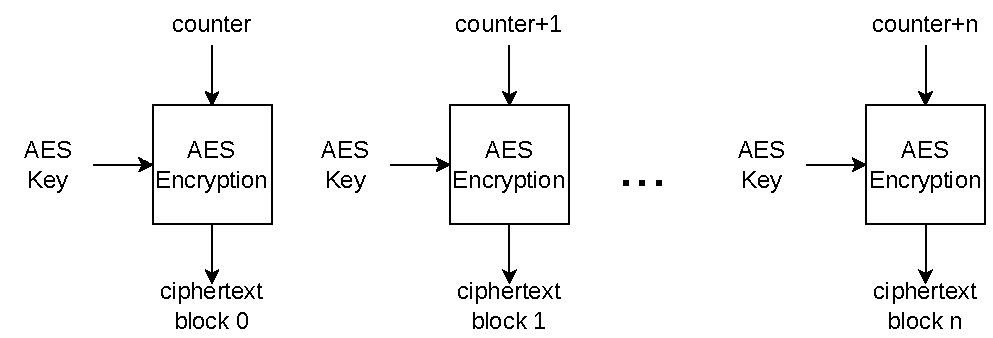
\includegraphics[width=1\linewidth]{Images/AES.pdf}
    \caption{AES-CTR Mode.}
    \label{fig::aes}
\end{figure}

When used as a pseudorandom byte generator, AES-CTR requires careful management of the key and counter values. In particular, counter blocks must never repeat under the same key, as reuse would produce identical keystream blocks and could compromise security. %Under these conditions, AES-CTR provides an efficient means of generating pseudorandom byte sequences for cryptographic applications, including sampling the polynomial coefficients required by lattice-based encryption schemes.

Since each counter block can be encrypted independently, CTR mode supports parallel processing, making it particularly suitable for architectures with dedicated vector AES instructions, such as our ARM Cortex-A55. %Furthermore, generating pseudorandom bytes does not require padding, as the output can be truncated to the desired length.

\section{ARMv8}

ARMv8~\cite{arm2023cortexa55} is a 64-bit architecture profile of the Arm architecture designed to support high-performance, general-purpose computing across a wide range of devices, from mobile and embedded systems to servers and high-performance computing platforms. It extends the earlier ARM architecture with the AArch64 execution state, providing a 64-bit instruction set, a larger address space, and improved support for modern operating systems and applications, while retaining compatibility with the 32-bit AArch32 execution state. In addition to the core instruction set, ARMv8 defines features for memory management, exception handling, virtualization, and security, providing the architectural foundation for modern Arm-based processors. The ARMv8 provide 32 128-bit Single-Instruction Multiple-Data (SIMD) registers through the ARM NEON extension, as well as optional dedicated cryptographic instructions for accelerating AES.

%Our target ARM Cortex A55 is ARMv8 compliant and has support to both ARM NEON and AES extensions. Furthermore, ARM Cortex A55 is a quad-core processor with the DynamicIQ technology, where each core has its own energy and frequency controller to dynamically select the operational frequency accordingly to the current workload. It core is a 8 stage pipeline and contain its own set of vector registers.


\subsection{ARM NEON}

The ARM NEON extension provides 32 128-bit vector registers and supports several classes of SIMD instructions, including vector–vector and vector–scalar arithmetic and logical operations on integer and floating-point data, vector permutation, bit manipulation (e.g., population count and bitwise operations), vector load and store operations, and cryptographic operations, such as AES instructions when the corresponding extension is available.

These instructions can be accessed from C code through function-like calls provided by the ARM NEON intrinsics library. Intrinsic names follow a naming convention in which suffixes indicate the vector width, the data type, and, when applicable, whether an operand is a scalar. For example, \texttt{vaddq\_s32} performs addition on 32-bit signed integers using 128-bit vectors, whereas \texttt{vmul\_f32} multiplies 32-bit floating-point values using 64-bit vectors. Similarly, \texttt{vaddq\_n\_u8} adds a scalar to each 8-bit unsigned integer element in a 128-bit vector.

The most relevant intrinsics for this work are listed below, with their suffixes omitted for simplicity.

\begin{itemize}
    \item \texttt{vld1}: Loads vector elements from memory into a SIMD register.

    \item \texttt{vst1}: Stores vector elements from a SIMD register to memory.

    \item \texttt{veor}: Performs element-wise XOR of vector elements.
    
    \item \texttt{vadd}: Performs element-wise addition of vector elements.
    
    \item \texttt{vsub}: Performs element-wise subtraction of vector elements.

    \item \texttt{vneg}: Performs element-wise negation of vector elements.
    
    \item \texttt{vmul}: Performs element-wise multiplication of vector elements.

    \item \texttt{vfma}: Performs element-wise fused multiplication and addition of vector elements.

    \item \texttt{vfms}: Performs element-wise fused multiplication and subtraction of vector elements.
    
    \item \texttt{vzip1}: Interleaves the lower elements of two vectors.
    
    \item \texttt{vzip2}: Interleaves the upper elements of two vectors.

    \item \texttt{vdup}: Propagate a constant to all vector elements.

    \item \texttt{vset\_lane}: Set one specific element of a vector to a constant.

    \item \texttt{vget\_low}: Obtain the lower 64-bit of a 128-bit vector register.

    \item \texttt{vget\_high}: Obtain the upper 64-bit of a 128-bit vector register.

    \item \texttt{vqtbl1}: Permutes the elements of the data source vector based on the index vector elements.

    \item \texttt{vext}: Extracts a sequence of consecutive elements from the concatenation of two vectors, starting from a given position to form the result vector.

    \item \texttt{vcnt}: Counts the number of set bits in each byte
    of a vector with 8-bit elements.
    
    \item \texttt{vsshll}: Sign-extends integer elements into elements
    of twice the width, optionally applying a left shift. The \texttt{vmovl} intrinsic is defined for the shift by zero case.

    \item \texttt{vaese}: Performs the AES \textbf{AddRoundKey}, \textbf{SubBytes}, \textbf{ShiftRows} operations using the vector register as AES state.

    \item \texttt{vaesmc}: Performs the AES \textbf{MixColumns} operation using the vector register as AES state.
    
\end{itemize}

In particular, NEON does not provide arithmetic intrinsics for 64-bit integer operands in all the required operations, which poses a significant challenge for this work, as each CRT modulus must be represented using 64-bit words.

\subsection{ARM Cortex-A55}

The target processor, the ARM Cortex-A55, implements the ARMv8-A architecture and supports both the ARM NEON SIMD instruction set and the AES cryptographic extension.      %NEON enables data-parallel processing by performing operations on multiple data elements within vector registers, making it suitable for accelerating computationally intensive workloads. The AES extension provides hardware instructions for accelerating AES encryption and decryption operations.
The Cortex-A55 is designed for energy-efficient performance in multicore systems and supports DynamIQ, ARM's technology for integrating Cortex processors into a shared processing cluster. In a quad-core configuration, the processor contains four cores, each with its own execution resources and architectural state, including its own set of NEON registers and level 1 and level 2 caches. The cores can operate at frequencies managed by the platform's power-management system, allowing performance and energy consumption to be adjusted according to workload demands.

Each Cortex-A55 core features an eight-stage pipeline for integer instructions and a ten-stage pipeline for floating-point and NEON instructions, allowing the processor to execute different classes of operations through dedicated datapaths. %Each core also maintains its own architectural register state, including the NEON register file, which contains thirty-two 128-bit vector registers in AArch64 execution state. These registers enable SIMD operations to process multiple data elements within a single instruction, which is particularly beneficial for the vectorized arithmetic operations investigated in this work. [Arm Documentation Service](https://documentation-service.arm.com/static/5f1fe66bbb903e39c84d7d75?utm_source=chatgpt.com)

%The Cortex-A55's support for the ARMv8-A architecture and its NEON and cryptographic extensions makes it a suitable target for evaluating SIMD optimizations. However, the exact number of cores, supported extensions, and available frequency-management capabilities depend on the specific system-on-chip (SoC) implementation. [Arm](https://www.arm.com/products/silicon-ip-cpu/cortex-a/cortex-a55?utm_source=chatgpt.com)

\section{OpenMP}

Open Multi-Processing (OpenMP) is an application programming interface (API) designed to facilitate shared-memory parallel programming in C, C++, and Fortran. It provides a set of compiler directives, runtime library routines, and environment variables that enable developers to parallelize a program with relatively small modifications to existing sequential code. Consequently, OpenMP provides a convenient approach for exploiting thread-level parallelism (TLP) and the multicore capabilities of the ARM Cortex-A55 processor for the CKKS operations considered in this work.

OpenMP follows a fork-join execution model, in which a master thread creates a team of worker threads to execute parallel regions and subsequently synchronizes with them at the end of the computation. This programming model makes OpenMP particularly suitable for exploiting multicore CPU architectures, as ARM Cortex-A55, where independent computations can be distributed among multiple processing cores to improve performance and reduce execution time. In this work, OpenMP is used to parallelize selected client-side operations, allowing the implementation to take advantage of the available CPU parallelism.

